\section{architecture}



%
% Graph representation
%
\begin{frame}\frametitle{Graph representation}

    \begin{itemize}
        \item \textbf{$G=(V, E)$} $\implies$ The graph represents the network
        \item \textbf{$v \in V$} $\implies$ Vertices represent \emph{Switches} and \emph{Hosts}
        \item \textbf{$u \to v \in E$} $\implies$  Edges represent \emph{links}
    \end{itemize}

\end{frame}


%
% Module atributes
%
\begin{frame}\frametitle{Graph representation}

    \begin{itemize}
        \item Vertices and Edges has extra data:
        \begin{itemize}
            \item Aplication expecific attributes
            \item Openflow counters collected from the switches
        \end{itemize}
        \item \emph{graph} abstraction uses information from POX's topology
            module 
    \end{itemize}

\end{frame}



%
% Pox design with our module
%
\begin{frame}\frametitle{Design}

	\begin{figure}[h]
        \centering
        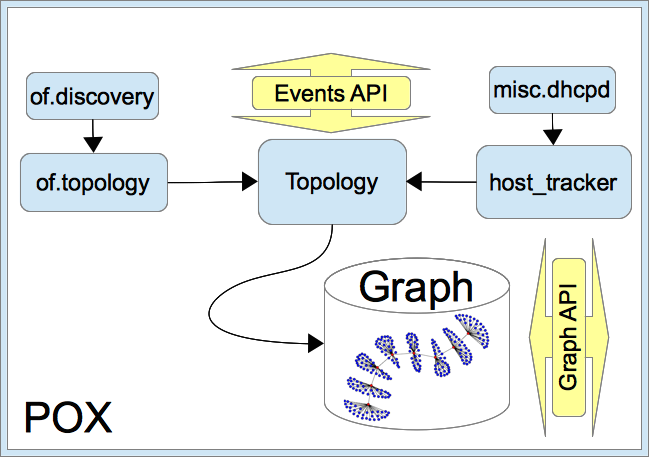
\includegraphics[scale=1.7]{img/design.png}
    \end{figure}
\end{frame}




%
% Experiments - Entity detection
%
\begin{frame}\frametitle{Entity detection}

    Performed by the \emph{topology} module
    \begin{itemize}
        \setlength{\itemsep}{10pt}
        \item Gets notifications from \emph{host\_tracker} and
            \emph{of.topology}
        \item Builds an event channel for updates
            \begin{itemize}
                \item join/leave events
                \item Other controller applications can listen to events they
                    care about
                \item Publisher/subscriber approach
            \end{itemize}
        \item Notifies join and leave of:
            \begin{itemize}
                \item Controller
                \item Switch
                \item Port
                \item Link
                \item Host
            \end{itemize}
    \end{itemize}
\end{frame}

%
% Experiments - Switches and Links
%
\begin{frame}\frametitle{Network devices detection}
    
    Performed by POX \emph{of.topology} module
    \begin{itemize}
        \item Uses LLDP to identify switches (POX's discovery class)
        \item Control informations about switches, links and ports
        \item Other modules may be created for other technologies
    \end{itemize}
\end{frame}


%
% Experiments - Host detection  
%
\begin{frame}\frametitle{Host detection}

    Performed by \emph{host\_tracker} module
    \begin{itemize}
        \item Listen to DHCP request/release messages
        \item Replaces ARP Protocol (answers to all requests)
    \end{itemize}
\end{frame}
